\documentclass[tikz,border=3pt]{standalone}
\usepackage{amsmath,amssymb}\usepackage{mathptmx}
\usepackage{tikz}
\usetikzlibrary{arrows.meta,positioning,fit,backgrounds,calc,shapes.geometric,decorations.pathreplacing}
\definecolor{ink}{HTML}{1F1F1E}
\definecolor{muted}{HTML}{5F5E58}
\definecolor{base}{HTML}{F3F3F1}
\definecolor{baseedge}{HTML}{8A8980}
\definecolor{newc}{HTML}{CDE2FB}
\definecolor{newedge}{HTML}{1C5CAB}
\definecolor{accent}{HTML}{EB6834}
\definecolor{accentlt}{HTML}{FBE1D6}
\tikzset{
  >={Stealth[length=2.2mm]},
  blk/.style={draw=baseedge, fill=base, rounded corners=2pt, align=center, font=\footnotesize,
              minimum height=10mm, inner sep=3pt, line width=0.5pt},
  newblk/.style={blk, draw=newedge, fill=newc, line width=0.8pt},
  accblk/.style={blk, draw=accent, fill=accentlt, line width=0.8pt},
  flow/.style={->, draw=ink, line width=0.6pt},
  newflow/.style={->, draw=newedge, line width=0.8pt, dashed},
  lbl/.style={font=\scriptsize, text=muted, align=center},
}

\begin{document}
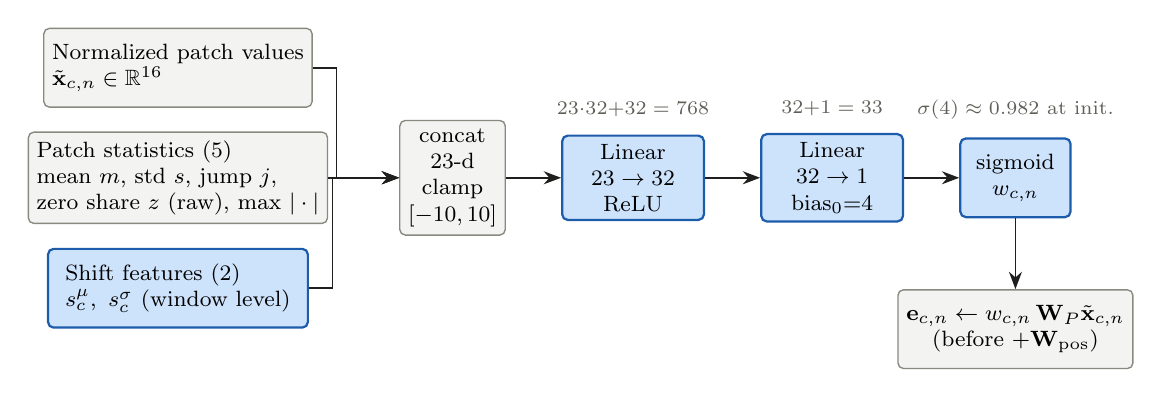
\begin{tikzpicture}[node distance=4mm and 7mm]
  % inputs
  \node[blk, minimum width=33mm, align=left] (pt) {Normalized patch values\\$\tilde{\mathbf{x}}_{c,n}\in\mathbb{R}^{16}$};
  \node[blk, minimum width=33mm, align=left, below=3mm of pt] (st) {Patch statistics (5)\\mean $m$, std $s$, jump $j$,\\zero share $z$ (raw), max $|\cdot|$};
  \node[newblk, minimum width=33mm, align=left, below=3mm of st] (sh) {Shift features (2)\\$s^{\mu}_c,\ s^{\sigma}_c$ (window level)};
  \node[blk, minimum width=12mm, right=9mm of st] (cat) {concat\\23-d\\clamp\\$[-10,10]$};
  \node[newblk, minimum width=18mm, right=of cat] (l1) {Linear\\$23\to32$\\ReLU};
  \node[newblk, minimum width=18mm, right=of l1] (l2) {Linear\\$32\to1$\\bias$_0{=}4$};
  \node[newblk, minimum width=14mm, right=of l2] (sig) {sigmoid\\$w_{c,n}$};
  \node[blk, minimum width=26mm, below=9mm of sig] (out) {$\mathbf{e}_{c,n}\leftarrow w_{c,n}\,\mathbf{W}_P\tilde{\mathbf{x}}_{c,n}$\\(before $+\mathbf{W}_{\text{pos}}$)};

  \draw[flow] (pt.east) -- ++(3mm,0) |- (cat.west);
  \draw[flow] (st.east) -- (cat.west);
  \draw[flow] (sh.east) -- ++(3mm,0) |- (cat.west);
  \draw[flow] (cat) -- (l1);
  \draw[flow] (l1) -- (l2);
  \draw[flow] (l2) -- (sig);
  \draw[flow] (sig) -- (out);
  \node[lbl, above=1mm of l1] {$23{\cdot}32{+}32=768$};
  \node[lbl, above=1mm of l2] {$32{+}1=33$};
  \node[lbl, above=1mm of sig] {$\sigma(4)\approx0.982$ at init.};
\end{tikzpicture}
\end{document}
